% ---
% titre: 9P - Lignes et surfaces
% theme: GM
% chapitre: Lignes et surfaces
% sous_chapitre:
% niveau: [9e]
% type: PLANIF
% tags: [c-conversion-unite,c-perimetre,c-aire]
% source: latex
% ---

\header{Lignes et surfaces - Objectifs}

\def\arraystretch{1.2}
\begin{tabularx}{\linewidth}{|>{\centering\arraybackslash}p{3cm}|>{\centering\arraybackslash}p{3cm}|X|}
\hline
\cellcolor{themeColor!30} Livre & \cellcolor{themeColor!30} Fiches & \cellcolor{themeColor!30} \hfill Aide-mémoire\hfill\null\\
\hline
&&Unités de mesure: pp. 170-176\\
pp. 149-164&pp. 183-196&Périmètre d'une surface: pp. 177-178\\
&&Aire d'une surface: pp. 179-182\\
\hline
\end{tabularx}
\def\arraystretch{1}

\def\arraystretch{1.6}
\begin{tabularx}{\textwidth}{|>{\raggedright\arraybackslash}X|>{\raggedright\arraybackslash}X|}
\hline
\cellcolor{themeColor!30}Compétences visées & \cellcolor{themeColor!30}Utilité dans la vie de tous les jours \\
\hline
Mobiliser les savoirs, savoir-faire et savoir être pour résoudre des problèmes en lien avec les lignes et les surfaces.
&\vspace{-1em}
\begin{itemize}[leftmargin=*, itemsep=2pt, topsep=0pt, partopsep=0pt, parsep=0pt, label=$\triangleright$]
    \item Voir dans l'esapce
    \item Agencer un appartement
    \item Construire un meuble
\end{itemize} \\
\hline

Développer des stratégies de recherche afin de résoudre des problèmes.
&\vspace{-1em}
\begin{itemize}[leftmargin=*, itemsep=2pt, topsep=0pt, label=$\triangleright$]
    \item Découper un projet en sous-tâches
    \item Choisir l'ordre des tâches à effectuer
\end{itemize} \\
\hline

Présenter sa démarche de façon claire (explications, grandeur cherchée, unités, calculs, réponse).
&\vspace{-1em}
\begin{itemize}[leftmargin=*, itemsep=2pt, topsep=0pt, label=$\triangleright$]
    \item Collaborer avec d'autres personnes
    \item Expliciter sa compréhension d'un sujet
    \item Argumenter
\end{itemize} \\
\hline

Développer des stratégies d'apprentissage pour s'approprier puis mobiliser les savoirs et savoir-faire.
&\vspace{-1em}
\begin{itemize}[leftmargin=*, itemsep=2pt, topsep=0pt, label=$\triangleright$]
    \item Apprendre une nouvelle activité %(art, sport, \ldots)
    \item S'adapter à un nouvel environnement %(travail, voyage, \ldots)
    \item Se former en autonomie %(tutoriel, lecture, \ldots)
\end{itemize} \\
\hline

Vérifier sa solution ou au moins sa plausibilité.
&\vspace{-1em}
\begin{itemize}[leftmargin=*, itemsep=2pt, topsep=0pt, label=$\triangleright$]
    \item S'autocritiquer
    \item Évaluer la qualité de son travail
\end{itemize} \\
\hline
\end{tabularx}
\def\arraystretch{1}

\newpage
\vfill
\def\arraystretch{1.6}
\begin{tabularx}{\textwidth}{|>{\raggedright\arraybackslash}p{5.2cm}|>{\raggedright\arraybackslash}X|>{\centering\arraybackslash}p{0.8cm}|>{\centering\arraybackslash}p{0.8cm}|>{\centering\arraybackslash}p{0.8cm}|}
\hline
\rowcolor{themeColor!30}\multicolumn{2}{|l|}{Objectifs} &\multicolumn{3}{c|}{Auto-évaluation} \\
\rowcolor{themeColor!30}\multicolumn{2}{|l|}{} & \Sadey[1.5]& \Neutrey[1.5] & \Smiley[1.5]  \\\hline

\multirow{3}{=}{Comparaison, classement et mesure de grandeurs par manipulation de lignes, angles, surfaces, en utilisant des unités conventionnelles et non conventionnelles}
& Comparer deux longueurs, deux angles ou deux surfaces sans les mesurer (par superposition, découpage, quadrillage, \ldots) & & & \\
\cline{2-5}
& Classer des longueurs, des angles ou des surfaces du plus petit au plus grand & & & \\
\cline{2-5}
& Mesurer une longueur, un angle ou une surface à l'aide d'une unité non conventionnelle (ex.: un gabarit, \ldots) & & & \\
\hline

\multirow{4}{=}{Estimation de grandeurs, choix d'une unité adéquate, prise de mesure à l'aide d'un instrument adapté et expression d'une grandeur avec des unités de longueur et d'aire}
& Estimer une longueur ou une aire avant de la mesurer (pièce de monnaie, feuille A4, salle de classe, terrain de foot, \ldots) & & & \\
\cline{2-5}
& Choisir l'unité la plus adaptée pour exprimer une longueur ou une aire donnée & & & \\
\cline{2-5}
& Connaître les unités de longueur et savoir les convertir & & & \\
\cline{2-5}
& Connaître les unités d'aire (notamment a et ha) et savoir les convertir & & & \\
\hline

\multirow{6}{=}{Mesure des dimensions adéquates et calcul :
\begin{itemize}[label=$\triangleright$]
    \item du périmètre d'un polygone
    \item de l'aire d'un carré, d'un rectangle, d'un triangle, d'un parallélogramme, d'un losange, d'un trapèze
    \item de l'aire d'un polygone par décomposition en figures simples
\end{itemize}}
& Différencier les concepts de périmètre et d'aire & & & \\
\cline{2-5}
& Mesurer les dimensions nécessaires sur une figure pour calculer son périmètre ou son aire & & & \\
\cline{2-5}
& Calculer le périmètre d'une figure par addition des longueurs qui le composent & & & \\
\cline{2-5}
& Connaître et utiliser les formules de périmètre des figures usuelles : carré, rectangle, triangle, parallélogramme, losange, trapèze & & & \\
\cline{2-5}
& Connaître et utiliser les formules d'aire des figures usuelles : carré, rectangle, triangle, parallélogramme, losange, trapèze & & & \\
\cline{2-5}
& Décomposer un polygone complexe en figures usuelles pour calculer son aire par addition ou soustraction & & & \\
\hline
\end{tabularx}
\def\arraystretch{1}
 \vfill

%------------------------------------------------
\newpage
\header{Lignes et surfaces - Feuille de route}

\newcommand{\rref}[1]{\textcolor{themeColor}{#1}}

% Case à cocher
\newcommand{\case}{\raisebox{-0.1ex}{\Large$\square$}}

% Marqueurs obligatoire / facultatif (forme, pas seulement couleur)
\newcommand{\oblig}{\tikz[baseline=-0.5ex]{\fill[themeColor] (0,0) circle (0.09);}}
\newcommand{\faclt}{\tikz[baseline=-0.5ex]{\draw[gray!70,line width=0.6pt] (0,0) circle (0.09);}}

 \vspace{20pt}
\begin{tikzpicture}[
circ/.style={circle, fill=themeColor, text=white, font=\bfseries\Large, minimum size=11mm, inner sep=0pt},
  box/.style={rectangle, draw=themeColor!35!white, rounded corners=2pt, fill=themeColor!8!white, inner sep=3mm, text width=14.7cm, align=left, anchor=north west}]

% ---------- Étape 1 ----------
\node[circ, anchor=north] (c1) at (0,0) {1};
\node[box] (b1) at ($(c1.north)+(1.2cm,0)$) {%
\textbf{\large Conversion d'unités}\\[4pt]
{\small\begin{tabularx}{10cm}{cXp{3cm}p{1cm}}
\case & \rref{Problème 60 A., D.} & VLM, p.\,49-50 & \oblig \\
\case & Problème 60 E., F. & VLM, p.\,49-50 & \faclt \\
\end{tabularx}}
};

% ---------- Étape 2 ----------
\coordinate (y2) at ($(b1.south west)+(0,-3mm)$);
\node[circ, anchor=north] (c2) at (c1 |- y2) {2};
\node[box] (b2) at (y2) {%
\textbf{\large Aire et périmètre}\\[4pt]
{\small\begin{tabularx}{10cm}{cXp{3cm}p{1cm}}
\case & \rref{GM 26}        & Livre, p.\,153 & \oblig \\
\case & \rref{GM 27}        & Livre, p.\,153 & \oblig \\
\case & \rref{Problème 92}  & VLM, p.\,75    & \oblig \\
\case & \rref{GM 36}        & Livre, p.\,157 & \oblig \\
\case & \rref{GM 33}        & Livre, p.\,155 & \oblig \\
\case & \rref{GM 34}        & Livre, p.\,156 & \oblig \\
\case & \rref{GM 49}        & Livre, p.\,161 & \oblig \\
\case & \rref{GM 52}        & Livre, p.\,162 & \oblig \\
\case & \rref{GM 51}        & Livre, p.\,162 & \oblig \\
\end{tabularx}}
};

% ---------- Étape 3 ----------
\coordinate (y3) at ($(b2.south west)+(0,-3mm)$);
\node[circ, anchor=north] (c3) at (c1 |- y3) {3};
\node[box] (b3) at (y3) {%
\textbf{\large Exercices \guillemotleft\,Défi\,\guillemotright}\\[4pt]
{\small\begin{tabularx}{10cm}{cXp{3cm}p{1cm}}
\case & GM 53      & Livre, p.\,163 & \faclt \\
\case & GM 50      & Livre, p.\,161 & \faclt \\
\case & Problème 89 & VLM, p.\,76   & \faclt \\
\end{tabularx}}
};

% ---------- Ligne de parcours (derrière les cercles) ----------
\begin{pgfonlayer}{background}
\draw[themeColor, line width=2pt] (c1) -- (c2) -- (c3);
\end{pgfonlayer}

\end{tikzpicture}

 \vfill
\begin{center}
\small \case~à faire \qquad \oblig~\rref{obligatoire} \qquad \faclt~facultatif (consolidation / pour aller plus loin)
\end{center}
\vspace{1em}


%------------------------------------------------
\newpage
\header{Lignes et surfaces - Théorie}

\subsection*{1. Unités de mesure}

\begin{regle}{Définition}
Une \textcolor{themeColor}{unité de mesure} est une grandeur de référence permettant de comparer des quantités. Elle est notée par une ou plusieurs lettres, par exemple kg.
\end{regle}


\vspace{20pt}
\def\arraystretch{2}
\begin{tabularx}{\linewidth}{|l|X|}
\hline
\rowcolor{themeColor!30}Grandeur physique & Exemples d'unités \\\hline
Longueur & mètre [m], kilomètre [km], millimètre [mm], \ldots \\\hline
Surface & mètre carré [m$^2$], kilomètre carré [km$^2$], \ldots \\\hline
Volume & mètre cube [m$^3$], millimètre cube [mm$^3$], \ldots \\\hline
Temps & seconde [s], minute [min], heure [h], jour [j], \ldots \\\hline
Masse & gramme [g], kilogramme [kg], tonne [t], \ldots \\\hline
Vitesse & kilomètre par heure [km/h], mètre par seconde [m/s], \ldots \\\hline
Température & degré Celsius [\textdegree{}C], Kelvin [K], \ldots \\\hline
Puissance & Watt [W], kilowatt [kW], gigawatt [GW], \ldots \\\hline
\end{tabularx}
\def\arraystretch{1}

\vfill
\begin{astuce}{Attention}
Les opérations $+$, $-$ et $=$ ne peuvent être appliquées qu'à condition de respecter deux règles :

\vspace{10pt}
\begin{enumerate}
    \item Les quantités doivent représenter la \textcolor{themeColor}{même grandeur physique} (deux longueurs, ou deux masses, mais jamais une longueur et une masse).
    \item Les quantités doivent être exprimées dans la \textcolor{themeColor}{même unité} (il faut d'abord convertir si besoin).
\end{enumerate}

\vspace{10pt}
Par exemple, $1\,\text{m} + 1\,\text{kg}$ n'a pas de sens : ce sont deux grandeurs physiques différentes.\\[7pt]
De même, $1\,\text{m} + 1\,\text{km}$ n'est pas correct tel quel : il faut d'abord convertir dans une unité commune, par exemple $1\,\text{m} + 1000\,\text{m} = 1001\,\text{m}$.
\end{astuce}

\newpage
\subsection*{2. Préfixes des unités de mesure}

Pour chaque unité, on peut ajouter un préfixe qui indique la taille de l'unité. Par exemple, un kilomètre correspond à 1\,000 mètres.

\vspace{10pt}
{\footnotesize
\def\arraystretch{2}
\begin{tabularx}{\linewidth}{|*{7}{C|}}
\hline
\rowcolor{themeColor!30}kilo- & hecto- & déca- & (unité) & déci- & centi- & milli- \\\hline
[k-] & [h-] & [da-] & [-] & [d-] & [c-] & [m-] \\\hline
$1\,000$ & $100$ & $10$ & $1$ & $0,1$ & $0,01$ & $0,001$ \\\hline
\end{tabularx}
\def\arraystretch{1}}

\vfill
\subsection*{3. Unité de distance}

Une distance est une longueur en ligne droite. Elle est exprimée en \textcolor{themeColor}{mètre, symbole m}.

\vspace{10pt}
{\footnotesize
\def\arraystretch{2}
\begin{tabularx}{\linewidth}{|*{7}{C|}}
\hline
km&hm&dam&\cellcolor{themeColor!30}m&dm&cm&mm\\\hline
$\cdot 1\,000$&$\cdot 100$&$\cdot 10$&\cellcolor{themeColor!30}$\cdot 1$&$\cdot 0,1$&$\cdot 0,01$&$\cdot 0,001$\\\hline
\end{tabularx}
\def\arraystretch{1}}

\vspace{20pt}
\begin{regle}{Définitions}
\textcolor{themeColor}{Convertir vers une unité plus petite}, c'est donner à chaque chiffre une valeur 10 fois plus petite (pour chaque colonne franchie vers la droite). Le nombre devient donc plus grand.\\[7pt]
\textcolor{themeColor}{Convertir vers une unité plus grande}, c'est donner à chaque chiffre une valeur 10 fois plus grande (pour chaque colonne franchie vers la gauche). Le nombre devient donc plus petit.
\end{regle}

\vspace{30pt}\begin{astuce}{Astuce}

\def\arraystretch{1.5}
\vspace{-5pt}\begin{tabularx}{\linewidth}{lX|lX}
\multicolumn{2}{l|}{Vers une unité plus \textbf{petite}}& \multicolumn{2}{l}{Vers une unité plus \textbf{grande}}\\\hline
1 colonne & $\cdot\, 10$ & 1 colonne & $:\, 10$ \\
2 colonnes & $\cdot\, 100$ & 2 colonnes & $:\, 100$ \\
3 colonnes & $\cdot\, 1000$ & 3 colonnes & $:\, 1000$ \\
\end{tabularx}
\def\arraystretch{1}

\vspace{10pt}
Le nombre de colonnes franchies dans le tableau des unités indique de combien de rangs chaque chiffre se déplace.
\end{astuce}

\newpage
Exemple: nous souhaitons convertir 24,5\,dam en cm.

\vspace{10pt}
\textcolor{themeColor}{Méthode par tableau}

1. Placer le chiffre de l'unité dans la colonne de l'unité de départ

{\footnotesize
\def\arraystretch{1.1}
\begin{tabularx}{\linewidth}{|*{7}{C|}}
\hline
km & hm & \cellcolor{themeColor!30}dam & m & dm & cm & mm \\\hline
&& 4 &&&& \\\hline
\end{tabularx}
\def\arraystretch{1}}

\vspace{10pt}
2. Réécrire le nombre de départ en plaçant un seul chiffre par case

{\footnotesize
\def\arraystretch{1.1}
\begin{tabularx}{\linewidth}{|*{7}{C|}}
\hline
km & hm & \cellcolor{themeColor!30}dam & m & dm &cm & mm \\\hline
& 2 & 4 & 5 &&& \\\hline
\end{tabularx}
\def\arraystretch{1}}

\vspace{10pt}
3. Repérer la colonne de l'unité d'arrivée

{\footnotesize
\def\arraystretch{1.1}
\begin{tabularx}{\linewidth}{|*{7}{C|}}
\hline
km & hm & dam & m & dm &\cellcolor{themeColor!30}cm & mm \\\hline
& 2 & 4 & 5 &&& \\\hline
\end{tabularx}
\def\arraystretch{1}}

\vspace{10pt}
4. Placer une virgule directement après la colonne de l'unité d'arrivée : c'est elle qui indique où se trouve désormais le chiffre des unités. Si des cases restent vides entre les chiffres du nombre et cette virgule, complète-les avec des zéros, puis enlève les zéros devenus inutiles

{\footnotesize
\def\arraystretch{1.1}
\begin{tabularx}{\linewidth}{|*{7}{C|}}
\hline
km & hm & dam & m & dm &\cellcolor{themeColor!30}cm & mm \\\hline
& 2 & 4 & 5 & 0 & \hspace{28pt}0 \hfill\textcolor{themeColor}{\textbf{,}}& \\\hline
\end{tabularx}
\def\arraystretch{1}}

\vspace{10pt}
5. Écrire le résultat

24,5\,dam = 24\,500\,cm

\vfill
\textcolor{themeColor}{Méthode directe}

1. Déterminer le sens : si l'unité d'arrivée est plus petite, on multiplie ; si elle est plus grande, on divise

cm < dam \quad$\Longrightarrow$\quad On multiplie.

\vspace{10pt}
2. Compter le nombre de rangs entre l'unité de départ et l'unité d'arrivée

dam $\xrightarrow{\times 10}$ m $\xrightarrow{\times 10}$ dm $\xrightarrow{\times 10}$ cm \quad$\Longrightarrow$\quad On bouge de trois rangs.

\vspace{10pt}
3. Multiplier ou diviser par $10$, $100$, $1000$, \ldots selon le nombre de rangs comptés à l'étape précédente

$24,5 \cdot 1000 = 24\,500$

\vspace{10pt}
4. Écrire le résultat

24,5\,dam = 24\,500\,cm

\newpage
\subsection*{4. Unité de surface}

Une surface est un espace en 2 dimensions. Elle est exprimée en \textcolor{themeColor}{mètre carré, symbole m$^2$}. $1\,\text{m}^2$ correspond à la surface couverte par un carré dont les côtés mesurent $1\,\text{m}$.

\vfill
\begin{center}
\begin{tikzpicture}[scale=1.6]
    % Carré hachuré
    \filldraw[themeColor!15, pattern=north east lines, pattern color=themeColor] (0,0) rectangle (1,1);
    \draw[themeColor, thick] (0,0) rectangle (1,1);

    % Label à l'intérieur
    \node at (0.5,0.5) {$1\,\text{m}^2$};

    % Côté du bas : 1 [m]
    \draw[<->, themeColor] (0,-0.25) -- (1,-0.25);
    \node[below] at (0.5,-0.25) {$1\,\text{m}$};

    % Côté droit : 1 [m]
    \draw[<->, themeColor] (1.25,0) -- (1.25,1);
    \node[right] at (1.25,0.5) {$1\,\text{m}$};
\end{tikzpicture}
\end{center}


\vfill
\begin{astuce}{Attention}
Comme $1\,\text{dam}^2 = 100\,\text{m}^2$, chaque colonne d'unité comporte \textcolor{themeColor}{deux sous-colonnes} plutôt qu'une seule.
\end{astuce}

\vspace{10pt}
{\footnotesize
\def\arraystretch{2}
\begin{tabularx}{\linewidth}{|*{14}{C|}}
\hline
\multicolumn{2}{|c|}{km$^2$}&\multicolumn{2}{c|}{hm$^2$}&\multicolumn{2}{c|}{dam$^2$}&\multicolumn{2}{c|}{\cellcolor{themeColor!30}m$^2$}&\multicolumn{2}{c|}{dm$^2$}&\multicolumn{2}{c|}{cm$^2$}&\multicolumn{2}{c|}{mm$^2$}\\\hline
\multicolumn{2}{|c|}{$\cdot 1\,000\,000$}&\multicolumn{2}{c|}{$\cdot 10\,000$}&\multicolumn{2}{c|}{$\cdot 100$}&\multicolumn{2}{c|}{\cellcolor{themeColor!30}$\cdot 1$}&\multicolumn{2}{c|}{$\cdot 0,01$}&\multicolumn{2}{c|}{$\cdot 0,0001$}&\multicolumn{2}{c|}{$\cdot 0,000001$}\\\hline
&&&&&&&&&&&&&\\\hline
\end{tabularx}
\def\arraystretch{1}}

\vspace{20pt}
\begin{regle}{Définitions}
\textcolor{themeColor}{Convertir vers une unité plus petite}, c'est donner à chaque chiffre une valeur 100 fois plus petite (pour chaque colonne franchie vers la droite). Le nombre devient donc plus grand.\\[7pt]
\textcolor{themeColor}{Convertir vers une unité plus grande}, c'est donner à chaque chiffre une valeur 100 fois plus grande (pour chaque colonne franchie vers la gauche). Le nombre devient donc plus petit.
\end{regle}

\vspace{30pt}\begin{astuce}{Astuce}

\def\arraystretch{1.5}
\vspace{-5pt}\begin{tabularx}{\linewidth}{lX|lX}
\multicolumn{2}{l|}{Vers une unité plus \textbf{petite}}& \multicolumn{2}{l}{Vers une unité plus \textbf{grande}}\\\hline
1 colonne & $\cdot\, 100$ & 1 colonne & $:\, 100$ \\
2 colonnes & $\cdot\, 10\,000$ & 2 colonnes & $:\, 10\,000$ \\
3 colonnes & $\cdot\, 1\,000\,000$ & 3 colonnes & $:\, 1\,000\,000$ \\
\end{tabularx}
\def\arraystretch{1}

\vspace{10pt}
Le nombre de colonnes franchies dans le tableau des unités indique de combien de rangs chaque chiffre se déplace — mais attention, chaque colonne compte pour \textcolor{themeColor}{deux} rangs (deux sous-colonnes) au lieu d'un seul.
\end{astuce}

\newpage
Exemple : nous souhaitons convertir $0,145\,\text{hm}^2$ en $\text{m}^2$.

\vspace{10pt}
\textcolor{themeColor}{Méthode par tableau}

1. Placer le chiffre des unités dans la case de droite de l'unité de départ

{\footnotesize
\def\arraystretch{1.1}
\begin{tabularx}{\linewidth}{|*{14}{C|}}
\hline
\multicolumn{2}{|c|}{km$^2$}&\multicolumn{2}{c|}{\cellcolor{themeColor!30}hm$^2$}&\multicolumn{2}{c|}{dam$^2$}&\multicolumn{2}{c|}{m$^2$}&\multicolumn{2}{c|}{dm$^2$}&\multicolumn{2}{c|}{cm$^2$}&\multicolumn{2}{c|}{mm$^2$}\\\hline
&&&0&&&&&&&&&&\\\hline
\end{tabularx}
\def\arraystretch{1}}

\vspace{10pt}
2. Réécrire le nombre de départ en plaçant un seul chiffre par case

{\footnotesize
\def\arraystretch{1.1}
\begin{tabularx}{\linewidth}{|*{14}{C|}}
\hline
\multicolumn{2}{|c|}{km$^2$}&\multicolumn{2}{c|}{\cellcolor{themeColor!30}hm$^2$}&\multicolumn{2}{c|}{dam$^2$}&\multicolumn{2}{c|}{m$^2$}&\multicolumn{2}{c|}{dm$^2$}&\multicolumn{2}{c|}{cm$^2$}&\multicolumn{2}{c|}{mm$^2$}\\\hline
&&&0&1&4&5&&&&&&&\\\hline
\end{tabularx}
\def\arraystretch{1}}

\vspace{10pt}
3. Repérer la case de droite de l'unité d'arrivée

{\footnotesize
\def\arraystretch{1.1}
\begin{tabularx}{\linewidth}{|*{14}{C|}}
\hline
\multicolumn{2}{|c|}{km$^2$}&\multicolumn{2}{c|}{hm$^2$}&\multicolumn{2}{c|}{dam$^2$}&\multicolumn{2}{c|}{\cellcolor{themeColor!30}m$^2$}&\multicolumn{2}{c|}{dm$^2$}&\multicolumn{2}{c|}{cm$^2$}&\multicolumn{2}{c|}{mm$^2$}\\\hline
&&&0&1&4&5&&&&&&&\\\hline
\end{tabularx}
\def\arraystretch{1}}

\vspace{10pt}
4. Placer une virgule directement après cette case. Compléter les cases vides entre les chiffres et cette virgule par des zéros, puis enlever les zéros devenus inutiles

{\footnotesize
\def\arraystretch{1.1}
\begin{tabularx}{\linewidth}{|*{14}{C|}}
\hline
\multicolumn{2}{|c|}{km$^2$}&\multicolumn{2}{c|}{hm$^2$}&\multicolumn{2}{c|}{dam$^2$}&\multicolumn{2}{c|}{\cellcolor{themeColor!30}m$^2$}&\multicolumn{2}{c|}{dm$^2$}&\multicolumn{2}{c|}{cm$^2$}&\multicolumn{2}{c|}{mm$^2$}\\\hline
&&&0&1&4&5&\hspace{10pt}0\hfill\textcolor{themeColor}{\textbf{,}}&&&&&&\\\hline
\end{tabularx}
\def\arraystretch{1}}

\vspace{10pt}
5. Écrire le résultat

0,145\,hm$^2$ = 1\,450\,m$^2$

\vfill
\textcolor{themeColor}{Méthode directe}

1. Déterminer le sens : si l'unité d'arrivée est plus petite, on multiplie; si elle est plus grande, on divise

$\text{m}^2 < \text{hm}^2 \quad\Longrightarrow\quad$ On multiplie.

\vspace{10pt}
2. Compter le nombre de rangs entre l'unité de départ et l'unité d'arrivée

hm$^2$ $\xrightarrow{\times 100}$ dam$^2$ $\xrightarrow{\times 100}$ m$^2$ $\quad\Longrightarrow\quad$ 2 colonnes vers la droite.

\vspace{10pt}
3. Multiplier ou diviser par $100$, $10\,000$, $1\,000\,000$, \ldots selon le nombre de rangs comptés à l'étape 2

$0,145 \cdot 10\,000 = 1\,450$

\vspace{10pt}
4. Écrire le résultat

0,145\,hm$^2$ = 1\,450\,m$^2$

\newpage
\subsection*{5. Périmètre et aire}

Pour n'importe quelle forme en deux dimensions, on définit les deux notions suivantes :

\vspace{20pt}
\begin{center}
\begin{tikzpicture}[scale=1.6]
    \def\forme{(0,0) -- (2,0) -- (2,1) -- (1.3,1) -- (1.3,1.8) -- (0,1.8) -- cycle}

    \filldraw[themeColor!15, pattern=north east lines, pattern color=themeColor] \forme;
    \draw[themeColor, ultra thick] \forme;

    \node[themeColor, fill=white, inner sep=2pt] at (0.65,1.1) {\small Aire};

    \node[themeColor, right] at (2.7,0.5) {\small Périmètre};
    \draw[themeColor, ->] (2.6,0.5) -- (2,0.5);
\end{tikzpicture}
\end{center}

\vspace{10pt}
\begin{regle}{Définitions}
Le \textcolor{themeColor}{périmètre} correspond à la longueur totale du contour de la forme. C'est une distance, notée $P$, exprimée en mètre.\\[7pt]
L'\textcolor{themeColor}{aire} correspond à la surface intérieure de la forme. C'est une surface, notée $A$, exprimée en mètre carré.
\end{regle}

\vspace{10pt}
\begin{astuce}{Attention}
Deux figures peuvent avoir la même aire sans avoir le même périmètre, et inversement. Ce sont deux grandeurs indépendantes.
\end{astuce}

\vfill
\subsection*{6. Périmètre et aire des figures usuelles}

\textcolor{themeColor}{Carré}

\begin{minipage}[c]{0.45\linewidth}
\begin{center}
\begin{tikzpicture}[scale=1]
	\tkzDefPoints{0/0/A,1.5/0/B, 1.5/1.5/C,0/1.5/D}
	\tkzDrawPolygon(A,B,C,D)
	\tkzLabelSegment[above,pos=.5](C,D){$c$}
	\tkzLabelSegment[left,pos=.5](A,D){$c$}
\end{tikzpicture}
\end{center}
\end{minipage}
\hfill
\begin{minipage}[c]{0.5\linewidth}
\begin{align*}
P &= c+c+c+c = 4\cdot c\\[6pt]
A &= c\cdot c = c^2
\end{align*}
\end{minipage}

\vspace{4pt}
{\small $c$ : mesure du côté}

\vspace{30pt}
\textcolor{themeColor}{Rectangle}

\begin{minipage}[c]{0.45\linewidth}
\begin{center}
\begin{tikzpicture}[scale=1]
	\tkzDefPoints{0/0/A,2/0/B, 2/1/C,0/1/D}
	\tkzDrawPolygon(A,B,C,D)
	\tkzLabelSegment[above,pos=.5](C,D){$L$}
	\tkzLabelSegment[left,pos=.5](A,D){$\ell$}
\end{tikzpicture}
\end{center}
\end{minipage}
\hfill
\begin{minipage}[c]{0.5\linewidth}
\begin{align*}
P &= L+\ell+L+\ell = 2\cdot(L+\ell)\\[6pt]
A &= L\cdot \ell
\end{align*}
\end{minipage}

\vspace{4pt}
{\small $L$ : mesure de la longueur\\
$\ell$ : mesure de la largeur}

\newpage
\textcolor{themeColor}{Parallélogramme}

\begin{minipage}[c]{0.45\linewidth}
\begin{center}
\begin{tikzpicture}[scale=1.3]
	\tkzDefPoints{0/0/A,3/0/B, 3.5/1.5/C,0.5/1.5/D}
	\tkzDrawPolygon(A,B,C,D)
	\tkzDefLine[perpendicular=through C](A,B)\tkzGetPoint{h1}\tkzInterLL(A,B)(C,h1)\tkzGetPoint{c}
	\tkzDefLine[orthogonal=through B](D,A)\tkzGetPoint{h2}\tkzInterLL(A,D)(B,h2)\tkzGetPoint{b}
	\tkzDrawSegment[dashed](C,c)\tkzDrawSegment[dashed](B,b)
	\tkzLabelSegment[right,pos=.5](C,c){$h_1$}\tkzLabelSegment[above right,pos=.5](B,b){$h_2$}
	\tkzLabelSegment[below,pos=.5](A,B){$b_1$}\tkzLabelSegment[left,pos=.5](A,D){$b_2$}
\end{tikzpicture}
\end{center}
\end{minipage}
\hfill
\begin{minipage}[c]{0.5\linewidth}
\begin{align*}
P &= b_1+b_2+b_1+b_2 = 2\cdot(b_1+b_2)\\[6pt]
A &= b_1\cdot h_1 = b_2\cdot h_2
\end{align*}
\end{minipage}

\vspace{4pt}
{\small $b_1, b_2$ : mesure des côtés\\
$h_1, h_2$ : mesure des hauteurs correspondantes}

\vfill
\textcolor{themeColor}{Losange}

\begin{minipage}[c]{0.45\linewidth}
\begin{center}
\begin{tikzpicture}[scale=1.3]
	\tkzDefPoints{0/0/A,2/-1/B, 4/0/C,2/1/D}
	\tkzDrawPolygon(A,B,C,D)
	\tkzLabelSegment[below left,pos=.5](A,B){$c$}
	\tkzDrawSegment[dashed,dim={$D$,50pt,midway,above=6pt},dim fence style/.append style={draw=none}](A,C)
	\tkzDrawSegment[dashed,dim={$d$,90pt,midway,left=6pt},dim fence style/.append style={draw=none}](B,D)
\end{tikzpicture}
\end{center}
\end{minipage}
\hfill
\begin{minipage}[c]{0.5\linewidth}
\begin{align*}
P &= c+c+c+c = 4\cdot c\\[6pt]
A &= \frac{D\cdot d}{2}
\end{align*}
\end{minipage}

\vspace{4pt}
{\small $c$ : mesure du côté\\
$D$ : mesure de la grande diagonale\\
$d$ : mesure de la petite diagonale}

\vfill
\textcolor{themeColor}{Trapèze}

\begin{minipage}[c]{0.45\linewidth}
\begin{center}
\begin{tikzpicture}[scale=1.3]
	\tkzDefPoints{0/0/A,4/0/B, 3/2/C,2/2/D}
	\tkzDrawPolygon(A,B,C,D)
	\tkzLabelSegment[below,pos=.5](A,B){$B$}\tkzLabelSegment[above,pos=.5](C,D){$b$}
	\tkzLabelSegment[left,pos=.5](A,D){$c_1$}\tkzLabelSegment[right,pos=.5](B,C){$c_2$}
	\tkzDefLine[perpendicular=through D](A,B)\tkzGetPoint{h1}\tkzInterLL(A,B)(D,h1)\tkzGetPoint{d}
	\tkzDrawSegment[dashed](D,d)\tkzLabelSegment[right,pos=.5](D,d){$h$}
\end{tikzpicture}
\end{center}
\end{minipage}
\hfill
\begin{minipage}[c]{0.5\linewidth}
\begin{align*}
P &= c_1+b+c_2+B\\[6pt]
A &= \frac{(B+b)\cdot h}{2} = \frac{(B+b)}{2}\cdot h
\end{align*}
\end{minipage}

\vspace{4pt}
{\small $B$ : mesure de la grande base \\
$b$ : mesure de la petite base\\
$h$ : mesure de la hauteur}

\vfill
\textcolor{themeColor}{Triangle}

\begin{minipage}[c]{0.45\linewidth}
\begin{center}
\begin{tikzpicture}[scale=1.3]
	\tkzDefPoints{0/0/A,4/0/B, 3/2/C}
	\tkzDrawPolygon(A,B,C)
	\tkzLabelSegment[above left,pos=.5](A,C){$b_1$}\tkzLabelSegment[below,pos=.5](A,B){$b_3$}\tkzLabelSegment[above right,pos=.5](B,C){$b_2$}
	\tkzDefLine[perpendicular=through B](A,C)\tkzGetPoint{h1}\tkzInterLL(A,C)(B,h1)\tkzGetPoint{b}
	\tkzDrawSegment[dashed,dim={$h_1$,-50pt,midway,above right=6pt},dim fence style/.append style={draw=none}](B,b)
	\tkzDefLine[perpendicular=through A](B,C)\tkzGetPoint{h2}\tkzInterLL(B,C)(A,h2)\tkzGetPoint{a}
	\tkzDrawSegment[dashed,dim={$h_2$,50pt,midway,below=6pt},dim fence style/.append style={draw=none}](A,a)
	\tkzDefLine[perpendicular=through C](A,B)\tkzGetPoint{h3}\tkzInterLL(A,B)(C,h3)\tkzGetPoint{c}
	\tkzDrawSegment[dashed,dim={$h_3$,-140pt,midway,left=6pt},dim fence style/.append style={draw=none}](C,c)
\end{tikzpicture}
\end{center}
\end{minipage}
\hfill
\begin{minipage}[c]{0.5\linewidth}
\begin{align*}
P &= b_1+b_2+b_3\\[6pt]
A &= \frac{b_1\cdot h_1}{2}=\frac{b_2\cdot h_2}{2}=\frac{b_3\cdot h_3}{2}
\end{align*}
\end{minipage}

\vspace{4pt}
{\small $b_1, b_2, b_3$ : mesure des bases\\
$h_1, h_2, h_3$ : mesure des hauteurs correspondantes}

\newpage
\subsection*{7. Périmètre et aire de figures complexes}

N'importe quelle figure peut être décomposée en plusieurs figures usuelles.

\vspace{15pt}
\begin{center}
\begin{tikzpicture}[scale=1.3]
    \def\forme{(0,0) -- (2,0) -- (2,1) -- (1.3,1) -- (1.3,1.8) -- (0,1.8) -- cycle}

    % Figure complexe
    \begin{scope}
        \draw[themeColor, ultra thick] \forme;
        \node[themeColor, below] at (1,-0.4) {\small Figure complexe};
    \end{scope}

    \node at (3,0.9) {\Large $=$};

    % Rectangle 1 (partie haute-gauche)
    \begin{scope}[xshift=3.7cm]
        \draw[themeColor, ultra thick] (0,0) rectangle (1.3,1.8);
        \node[themeColor, below] at (0.65,-0.4) {\small Rectangle 1};
    \end{scope}

    \node at (5.6,0.9) {\Large $+$};

    % Rectangle 2 (partie basse-droite)
    \begin{scope}[xshift=6cm]
        \draw[themeColor, ultra thick] (0,0) rectangle (0.7,1);
        \node[themeColor, below] at (0.35,-0.4) {\small Rectangle 2};
    \end{scope}
\end{tikzpicture}
\end{center}

\vfill
\subsubsection*{Aire}

\begin{regle}{Règle}
L'\textcolor{themeColor}{aire} d'une figure complexe est la \textbf{combinaison des aires} des figures usuelles qui la composent (par addition ou soustraction).
\end{regle}

\vspace{15pt}
\begin{center}
\begin{tikzpicture}[scale=1.3]
    \def\forme{(0,0) -- (2,0) -- (2,1) -- (1.3,1) -- (1.3,1.8) -- (0,1.8) -- cycle}

    \begin{scope}
        \filldraw[themeColor!15, pattern=north east lines, pattern color=themeColor] \forme;
        \draw[themeColor, thick] \forme;
        \node[themeColor, fill=white, inner sep=2pt] at (1,0.5) {\small $A$};
    \end{scope}

    \node at (3,0.9) {\Large $=$};

    \begin{scope}[xshift=3.7cm]
        \filldraw[themeColor!15, pattern=north east lines, pattern color=themeColor] (0,0) rectangle (1.3,1.8);
        \draw[themeColor, thick] (0,0) rectangle (1.3,1.8);
        \node[themeColor, fill=white, inner sep=2pt] at (0.65,0.9) {\small $A_1$};
    \end{scope}

    \node at (5.6,0.9) {\Large $+$};

    \begin{scope}[xshift=6cm]
        \filldraw[themeColor!15, pattern=north east lines, pattern color=themeColor] (0,0) rectangle (0.7,1);
        \draw[themeColor, thick] (0,0) rectangle (0.7,1);
        \node[themeColor, fill=white, inner sep=2pt] at (0.35,0.5) {\small $A_2$};
    \end{scope}
\end{tikzpicture}
\end{center}

\begin{center}
$A = A_1 + A_2$
\end{center}

\vfill
\subsubsection*{Périmètre}

\begin{regle}{Règle}
Pour calculer le périmètre d'une figure complexe, il suffit d'\textbf{additionner les longueurs des segments} qui forment son contour.
\end{regle}

\vspace{15pt}
\begin{center}
\begin{tikzpicture}[scale=1.3]
    \def\forme{(0,0) -- (2,0) -- (2,1) -- (1.3,1) -- (1.3,1.8) -- (0,1.8) -- cycle}

    \begin{scope}
        \draw[themeColor, ultra thick] \forme;
        \node[themeColor, fill=white, inner sep=2pt] at (1,0.5) {\small $P$};
    \end{scope}

    \node at (3,0.9) {\Large $\neq$};

    \begin{scope}[xshift=3.7cm]
        \draw[themeColor, ultra thick] (0,0) rectangle (1.3,1.8);
        \node[themeColor, fill=white, inner sep=2pt] at (0.65,0.9) {\small $P_1$};
    \end{scope}

    \node at (5.6,0.9) {\Large $+$};

    \begin{scope}[xshift=6cm]
        \draw[themeColor, ultra thick] (0,0) rectangle (0.7,1);
        \node[themeColor, fill=white, inner sep=2pt] at (0.35,0.5) {\small $P_2$};
    \end{scope}
\end{tikzpicture}
\end{center}

\vspace{10pt}
\begin{astuce}{Attention}
Le \textcolor{themeColor}{périmètre} d'une figure complexe n'est \textbf{pas} la combinaison des périmètres des figures usuelles qui la composent.
\end{astuce}

%------------------------------------------------
\newpage
\header{Lignes et surfaces - Lexique}

\newtcolorbox{terme}{%
  enhanced, sharp corners, boxrule=0pt, colback=themeColor!6!white,
  colframe=themeColor!6!white,
  borderline west={2.2pt}{0pt}{themeColor},
  left=3mm, right=2mm, top=2mm, bottom=2mm,
}

 \vfill
\begin{tcbraster}[raster columns=2, raster equal height, raster valign=top,raster column skip=2mm, raster row skip=2mm]
\begin{terme}
\textbf{\large Aire}\\[2pt]
{\small Surface intérieure d'une figure. Notée $A$, exprimée en mètre-carré [m$^2$].}
\end{terme}
\begin{terme}
\textbf{\large Base}\\[2pt]
{\small Côté d'une figure servant de référence pour calculer une hauteur correspondante.}
\end{terme}
\begin{terme}
\textbf{\large Carré}\\[2pt]
{\small Quadrilatère ayant 4 côtés isométriques et 4 angles droits.}
\end{terme}
\begin{terme}
\textbf{\large Conversion d'unité}\\[2pt]
{\small Passage d'une unité de mesure à une autre pour exprimer la même grandeur.}
\end{terme}
\begin{terme}
\textbf{\large Côté}\\[2pt]
{\small Segment qui forme le contour d'une figure.}
\end{terme}
\begin{terme}
\textbf{\large Diagonale}\\[2pt]
{\small Segment reliant deux sommets non consécutifs d'un polygone.}
\end{terme}
\begin{terme}
\textbf{\large Distance}\\[2pt]
{\small Longueur en ligne droite entre deux points. Exprimée en mètre [m].}
\end{terme}
\begin{terme}
\textbf{\large Figure complexe}\\[2pt]
{\small Figure qui peut être décomposée en plusieurs figures usuelles.}
\end{terme}
\begin{terme}
\textbf{\large Figure usuelle}\\[2pt]
{\small Figure de base : carré, rectangle, triangle, parallélogramme, losange ou trapèze.}
\end{terme}
\begin{terme}
\textbf{\large Grandeur}\\[2pt]
{\small Ce que l'on peut mesurer, par exemple une longueur, une aire, une masse ou un temps.}
\end{terme}
\begin{terme}
\textbf{\large Hauteur}\\[2pt]
{\small Segment perpendiculaire à une base, reliant celle-ci à un sommet opposé.}
\end{terme}
\begin{terme}
\textbf{\large Longueur}\\[2pt]
{\small Mesure d'une distance selon une direction donnée.}
\end{terme}
\begin{terme}
\textbf{\large Losange}\\[2pt]
{\small Quadrilatère ayant 4 côtés isométriques.}
\end{terme}
\begin{terme}
\textbf{\large Parallèle}\\[2pt]
{\small Se dit de deux droites (ou segments) qui ne se croisent jamais, aussi loin qu'on les prolonge.}
\end{terme}
\begin{terme}
\textbf{\large Parallélogramme}\\[2pt]
{\small Quadrilatère dont les côtés opposés sont parallèles deux à deux.}
\end{terme}
\begin{terme}
\textbf{\large Périmètre}\\[2pt]
{\small Longueur totale du contour d'une figure. Noté $P$, exprimé en mètre [m].}
\end{terme}
\begin{terme}
\textbf{\large Perpendiculaire}\\[2pt]
{\small Se dit de deux droites (ou segments) qui se croisent en formant un angle droit.}
\end{terme}
\begin{terme}
\textbf{\large Polygone}\\[2pt]
{\small Figure plane fermée, délimitée par des segments de droite appelés côtés.}
\end{terme}
\begin{terme}
\textbf{\large Préfixe}\\[2pt]
{\small Petit mot ajouté devant une unité pour en indiquer la taille (kilo-, centi-, \ldots).}
\end{terme}
\begin{terme}
\textbf{\large Quadrilatère}\\[2pt]
{\small Polygone ayant 4 côtés.}
\end{terme}
\begin{terme}
\textbf{\large Rectangle}\\[2pt]
{\small Quadrilatère ayant 4 angles droits.}
\end{terme}
\begin{terme}
\textbf{\large Sommet}\\[2pt]
{\small Point où se rencontrent deux côtés d'un polygone.}
\end{terme}
\begin{terme}
\textbf{\large Surface}\\[2pt]
{\small Espace en deux dimensions. Exprimée en mètre-carré [m$^2$].}
\end{terme}
\begin{terme}
\textbf{\large Trapèze}\\[2pt]
{\small Quadrilatère ayant une seule paire de côtés parallèles.}
\end{terme}
\begin{terme}
\textbf{\large Triangle}\\[2pt]
{\small Polygone à 3 côtés.}
\end{terme}
\begin{terme}
\textbf{\large Unité de mesure}\\[2pt]
{\small Grandeur de référence permettant de comparer des quantités.}
\end{terme}
\end{tcbraster}